\documentclass[a4paper]{article}
\addtolength{\hoffset}{-2.25cm}
\addtolength{\textwidth}{4.5cm}
\addtolength{\voffset}{-3.25cm}
\addtolength{\textheight}{5cm}
\setlength{\parindent}{15pt}

\usepackage[unicode=true, colorlinks=false, hidelinks]{hyperref}
\usepackage[utf8]{inputenc}
\usepackage[english, russian]{babel}
\usepackage{mathtext}
\usepackage[T2A, TS1]{fontenc}
\usepackage{microtype} % Slightly tweak font spacing for aesthetics
\usepackage{amsthm, amssymb, amsmath, amsfonts, nccmath}
\usepackage{nicefrac}
\usepackage{epstopdf}
\usepackage[export]{adjustbox}
\usepackage{float} % Improved interface for floating objects
\usepackage{graphicx, multicol} % Enhanced support for graphics
\usepackage{pdfrender,xcolor}
\usepackage{breqn}
\usepackage{mathtools}
\usepackage{titling}
\usepackage{bm}
\usepackage{centernot}
\usepackage[cal=boondoxo,calscaled=.96]{mathalpha}
\usepackage{marvosym, wasysym} % More symbols
\usepackage{rotating} % Rotation tools
\usepackage{censor} % Facilities for controlling restricted text
\usepackage{indentfirst}
\usepackage{svg}

\DeclareMathOperator{\rad}{rad}
\DeclareMathOperator{\imid}{mid}
\DeclareMathOperator{\sign}{sign}
\newcommand{\mbb}[1]{\mathbb{#1}}
\newcommand{\mbf}[1]{\mathbf{#1}}

\usepackage{array}
\newcolumntype{C}[1]{>{\centering\let\newline\\\arraybackslash\hspace{0pt}}m{#1}}

\usepackage{fancyhdr}
\pagestyle{fancy}
\fancyhead{}\renewcommand{\headrulewidth}{0pt}
\fancyfoot[L]{}
\fancyhead{}
\fancyfoot{}
\fancyfoot[R]{\thepage}
\begin{document}
\large
\begin{center}
    Санкт-Петербургский политехнический университет\\
    Высшая школа прикладной математики и\\вычислительной физики,\\ 
    Физико-механический институт\\
    \vspace{3em}
    Направление подготовки\\
    01.03.02 «Прикладная математика и информатика»\\
    \vspace{10em}
    \Large
    Отчет по лабораторной работе №4 \\
    по дисциплине «Интервальный анализ»
    \vspace{19em}
    \large
\end{center}
Выполнил студент гр. 5030102/80201\\
Кирпиченко С. Р.\\
Руководитель\\
Баженов А. Н.
\vspace{10em}
\begin{center}
    Санкт-Петербург\\
    2021
\end{center}
\thispagestyle{empty}
\newpage
\tableofcontents
\addtocontents{toc}{~\hfill\textbf{Страница}\par}
\newpage
\listoffigures
\addtocontents{lof}{~\hfill\textbf{Страница}\par}
\newpage
\section{Постановка задачи}
\subsection{Использование теоремы Зюзина}
Дана ИСЛАУ 
\begin{equation}\label{islau zuzin}
    \begin{cases}
    [1,\:4]\cdot x_1+[0.5,\:0.7]\cdot x_2=[-1,\:1]\\
    [0.8,\:1.2]\cdot x_1 + [3,\:5]\cdot x_2=[-3,\:3]
    \end{cases}
\end{equation}
Для нее необходимо построить итерационную схему с разложением матрицы на диагональную и недиагональную части по теореме Зюзина, а также провести вычисления и привести иллюстрации:
\begin{itemize}
    \item Брусов итерационного процесса
    \item Радиусов решения в зависимости от номера итерации
\end{itemize}
\subsection{Использование субдифференциального метода Ньютона}
Даны две ИСЛАУ:
\begin{equation}\label{islau new1}
    \begin{cases}
    [3,\:4]\cdot x_1+[5,\:6]\cdot x_2=[-3,\:3]\\
    [-1,\:1]\cdot x_1 + [-3,\:1]\cdot x_2=[-1,\:2]
    \end{cases}
\end{equation}
\begin{equation}\label{islau new2}
    \begin{cases}
    [3,\:4]\cdot x_1+[5,\:6]\cdot x_2=[-3,\:4]\\
    [-1,\:1]\cdot x_1 + [-3,\:1]\cdot x_2=[-1,\:2]
    \end{cases}
\end{equation}
Необходимо построить итерационную схему субдифференциального метода Ньютона, провести вычисления и привести иллюстрации брусов итерационного процесса, а также сравнить полученные результаты для систем (\ref{islau new1}) и (\ref{islau new2}).
\section{Теория}
\subsection{Теорема Зюзина}
Пусть в интервальной линейной системе уравнений 
$$\mbf{C}x=\mbf{d},\quad \mbf{C}\in\mbb{KR}^{n\times n},\:\mbf{d}\in\mbb{KR}^n$$
правильная проекция матрицы $\mbf{C}$ имеет диагональное преобладание. Тогда формальное решение системы существует и единственно.

Итерационный процесс строится следующим образом
$$\mbf{D}=\mathrm{diag}\{\mbf{c}_{ii}\}_{i=1}^n\quad\mbf{E}=\mbf{C}\ominus\mbf{D}$$
$$\mbf{C}x=\mbf{d}\Leftrightarrow\mbf{D}x=\mbf{d}\ominus\mbf{E}x$$
$$\mbf{x}^{k+1}=\mathrm{inv}\:\mbf{D}\cdot(\mbf{d}\ominus\mbf{E}\mbf{x}^k),\;k=0,1,\dots$$
\subsection{Субдифференциальный метод Ньютона}
Итерационная процедура субдифференциального метода Ньютона описывается следующей формулой:
$$x^k=x^{k-1}-\tau(D^{k-1})^{-1}\mathcal{F}(x^{k-1}),$$
где $\mathcal{F}(x)=\mathrm{sti}\:(\mbf{C}\cdot\mathrm{sti}^{-1}\:(x))-x+\mathrm{sti}\:(\mbf{d)}$ ($\mathrm{sti}$ - операция стандартного погружения, отображения из $\mbb{KR}^n$ в $\mbb{R}^{2n}$), $D^{k-1}$ - какой-нибудь субградиент отображения $\mathcal{F}$ в точке $x^{k-1}$, $\tau$ - константа, в данной работе выбрана единицей.
\section{Реализация}
Для осуществления вычислений и визуализации результатов использовалась среда Octave с библиотекой полной интервальной арифметики kinterval. 
\section{Результаты}
\subsection{Итерационный процесс с разложением матрицы на диагональную и недиагональную части}
Здесь и далее пунктиром обозначено допусковое множество $\Xi_{\mathrm{tol}}$ рассматриваемой ИСЛАУ. Также здесь и далее начальный брус обозначен синим цветом. Число итераций - 10.
\begin{figure}[H]
    \centering
    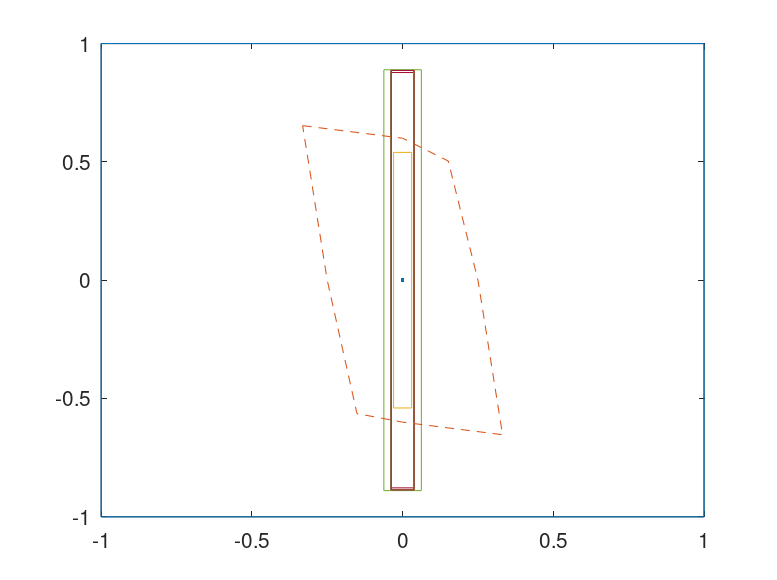
\includegraphics[width=11cm]{img/1_box.png}
    \caption{Изображение брусов при решении задачи (\ref{islau zuzin})}
    \label{fig:box_z}
\end{figure}
\begin{figure}[H]
    \centering
    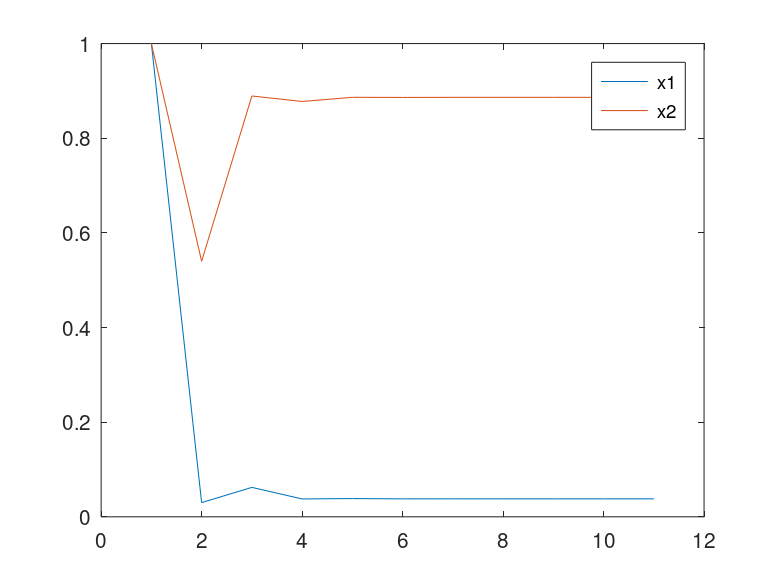
\includegraphics[width=11cm]{img/1_rads.png}
    \caption{Зависимость радиусов брусов от числа итераций при решении задачи (\ref{islau zuzin})}
    \label{fig:rad_z}
\end{figure}
\subsection{Итерационный процесс по субградиентному методу Ньютона}
Здесь и далее брусы, полученные по мере итераций обозначены пунктирными линиями с мелкой штриховкой, последний брус - сплошной линией красного цвета. При решении задачи ($\ref{islau new1}$) использовался параметр $\tau=1$, финальный брус получен на четвертой итерации метода. 
\begin{figure}[H]
    \centering
    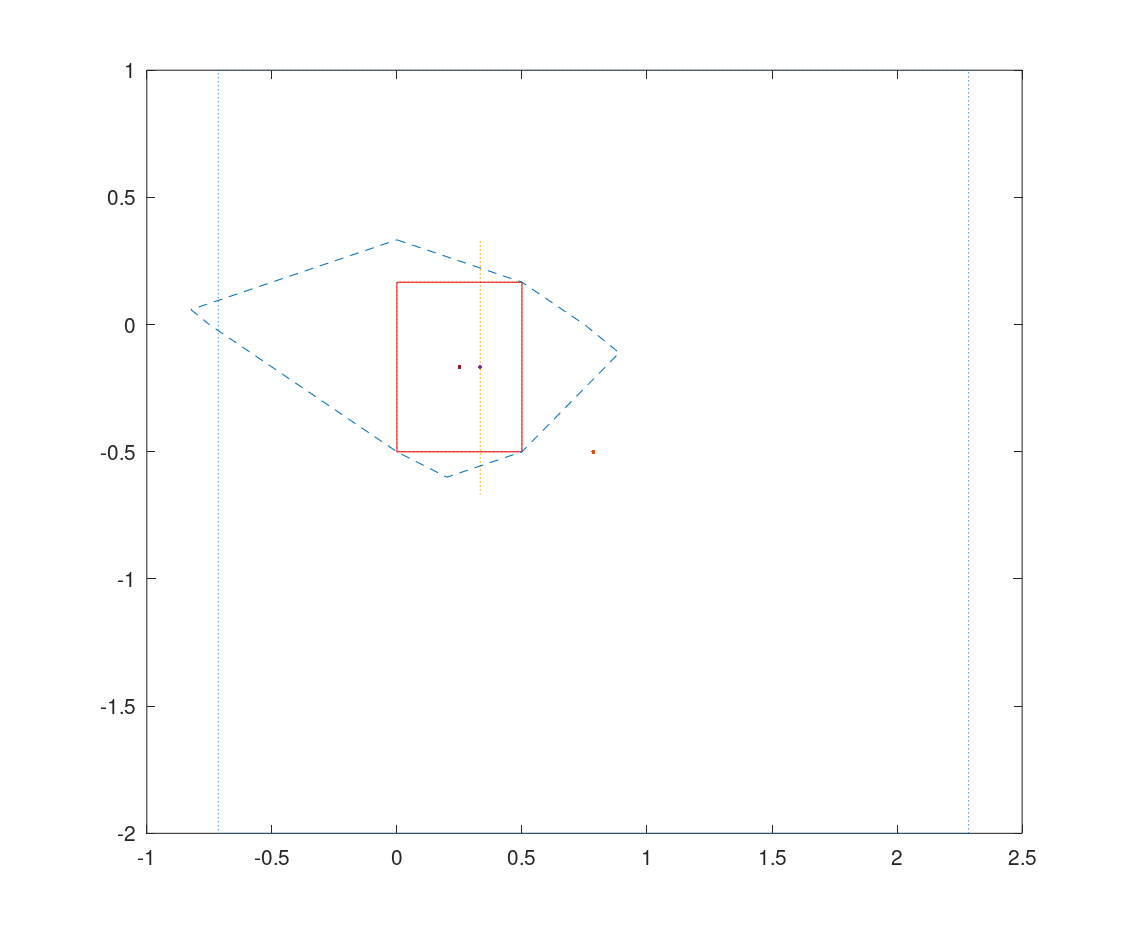
\includegraphics[width=11.5cm]{img/2_1.png}
    \caption{Решение задачи ($\ref{islau new1}$) субградиентным методом Ньютона, $\tau=1$}
    \label{fig:new_1}
\end{figure}
Решение задачи ($\ref{islau new2}$) с параметром $\tau=1$. Число итераций - 300.
\begin{figure}[H]
    \centering
    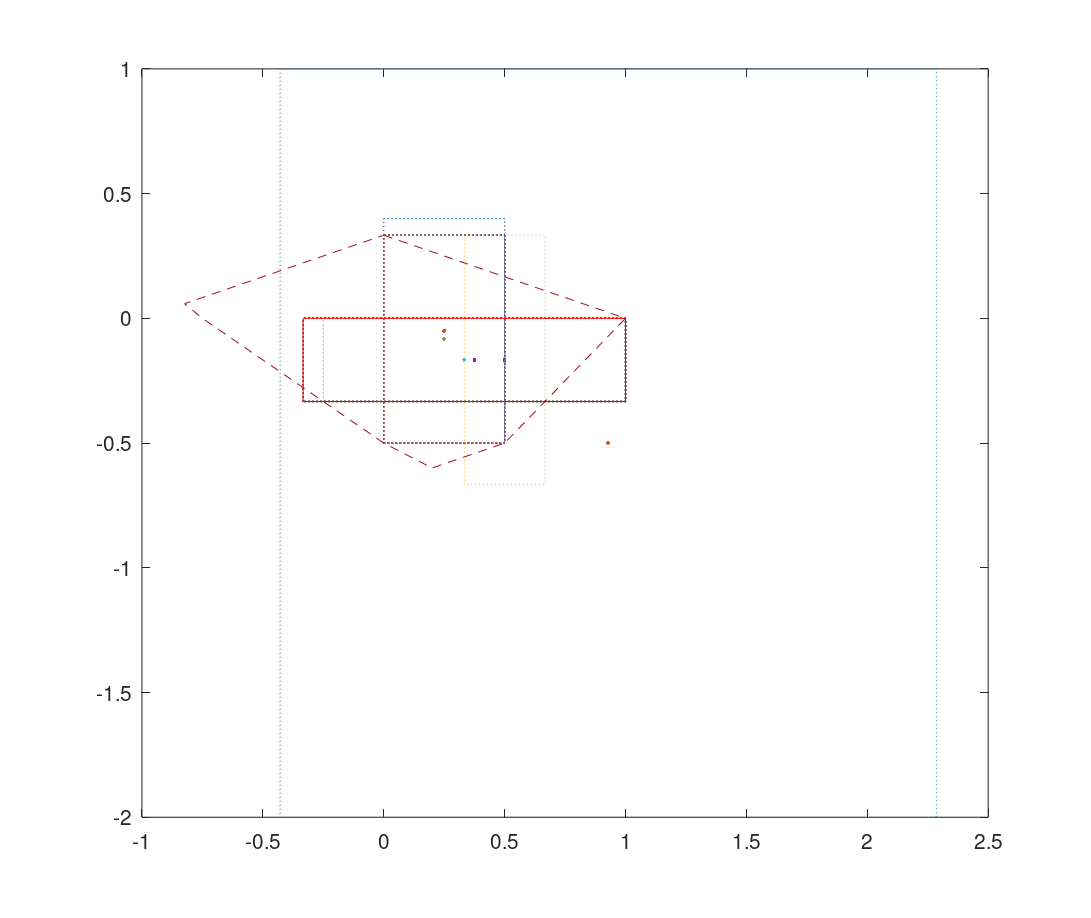
\includegraphics[width=11.5cm]{img/2_2_1.png}
    \caption{Решение задачи ($\ref{islau new2}$) субградиентным методом Ньютона, $\tau=1$}
    \label{fig:new_2_1}
\end{figure}
Решение задачи ($\ref{islau new2}$) с параметром $\tau=0.05$. Число итераций - 300.
\begin{figure}[H]
    \centering
    \includegraphics[width=15cm]{img/2_2_005.png}
    \caption{Решение задачи ($\ref{islau new2}$) субградиентным методом Ньютона, $\tau=0.05$}
    \label{fig:new_2_005}
\end{figure}
\section{Обсуждение}
\begin{enumerate}
    \item Сопоставляя графики \ref{fig:box_z} и \ref{fig:rad_z}, обнаруживаем, что на второй итерации метод выдал более адекватную внутреннюю оценку $\Xi_{\mathrm{tol}}$, чем на последней. Финальный результат выходит за пределы допускового множества. Середина брусов практически не меняется по мере итераций. После пятой итерации наблюдается стагнация в размере брусов.
    \item При решении задачи \ref{islau new1} получена точная внутренняя оценка $\Xi_{\mathrm{tol}}$, субградиентный метод Ньютона сошелся очень быстро - после четвертой итерации итерационный процесс остановился.
    \item При решении задачи \ref{islau new2} не была получена внутренняя оценка $\Xi_{\mathrm{tol}}$. Тем не менее, результат адекватный - около 85\% площади полученного бруса находится внутри допускового множества. Метод проделал все 300 итераций вплоть до заданных извне ограничений.
    \item При уменьшении параметра $\tau$ получен другой брус. Он все еще не является строгой внутренней оценкой $\Xi_{\mathrm{tol}}$, но эта оценка более удачна, так как полученный брус больше по площади, чем предыдущий, и еще большая его часть лежит внутри допускового множества. 
    \item С меньшим параметром $\tau$ изменение брусов по мере итераций меньше, эти изменения более плавные. Судя по графику \ref{fig:new_2_005}, можно предположить, что при устремлении числа итераций к бесконечности, все же можно получить точную внутреннюю оценку. Такой вывод нельзя сделать, опираясь на график \ref{fig:new_2_1}.
\end{enumerate}
\section*{Исходный код}
С исходным кодом программы и отчета можно ознакомиться в репозитории \url{https://github.com/Stasychbr/IntervalArith}.
\end{document}
